\documentclass{article}
\usepackage{../../fasy-hw}
\usepackage{ wasysym }

%% UPDATE these variables:
\renewcommand{\hwnum}{09}
\title{Discrete Structures, Misc 09}
\author{Patrick O'Connor}
\collab{n/a}
\date{due: 26 April 2021}

\begin{document}

\maketitle

This homework assignment should be
submitted as a single PDF file both to D2L and to Gradescope.

General homework expectations:
\begin{itemize}
    \item Homework should be typeset using LaTex.
    \item You will not plagiarize.
    \item List collaborators at the start of each question using the
        \texttt{collab} command.
    \item What did you learn?
    \item     What is a piece of advise that you took away?
    \item     Did an audience member ask a question that you particularly liked or disliked?
    \item    Is there a question that you wish you could have asked but didn't?
    \item     If related to the event, what were you thinking about as you were leaving?
    \item   Did this event inspire you to look something up after the event? If so, what was it?
    \item    Did you meet someone new at this event who you could see as a mentor / mentee / collaborator in the future?
    \item     What is your take-away message from this event?
    \item    How did the contents of this event relate to our class? (Even if not explicitly discussed).
\end{itemize}

% ============================================
% ============================================
\nextprob{Article in the News}
\collab{n/a}
% ============================================
% ============================================

Find a reference (direct or indirect) of something 
relating to this class in the news. Was the concept used or applied correctly? Using this article, 
explain the concept to your imaginary 8-year-old sibling.

The article that I found through a bit of researching is on the four-color thereom and a mistake that the author made when thinking about this 
thereom. This version that is linked below is an updated article that she created after a reader reached out to him via email. The reader 
noticed a flaw in her reasoning in that stated that "I talked about some of the hypotheses of the theorem, including the fact that countries 
or states need to be connected in order for the theorem to apply. In other words, we aren't guaranteed to be able to color a map with only 
four colors if I demand that both the Upper Peninsula and "mitten" of Michigan be colored green. I also said, "It was a little harder to 
figure out that a country shouldn’t have a hole in it, or completely surround another country or countries.". 

Simply put she believe that there had been a mistake in the four color thereom as when there is a hole in the country there would not be 
a four coloring. This is false as the reader justified with the stating the four-color theorem is not exactly about maps and globes as 
humans generally think about them but rather an interpertation in that the details are stripped away and we are left with only edges 
and vertices that represent the borders of each country. The reader also clarified that a graph that comes from a map will always be 
planar with no two edges connecting to vertices of the same color. 

Overall, the original post that the author had written had many flaws in it that did not align with what we have been learning throughout 
this class. But I did like that the author retracted his previous post and edited it to fit the mathematical standards for creating maps/graphs 
that are used when establishing four colorability. This revision does align with everything we are learning and is solid in following the correct 
guidelines. 

After reading this, I realize that although something is coming from a trusted journal such as the Scientific American there may be mistakes 
in the logic the author is using and it is best to use multiple sources when determining the reliability of a paper. 


\emph{Scientific American}~\cite{science}
\emph{Princeton}~\cite{princeton}

\begin{figure}
    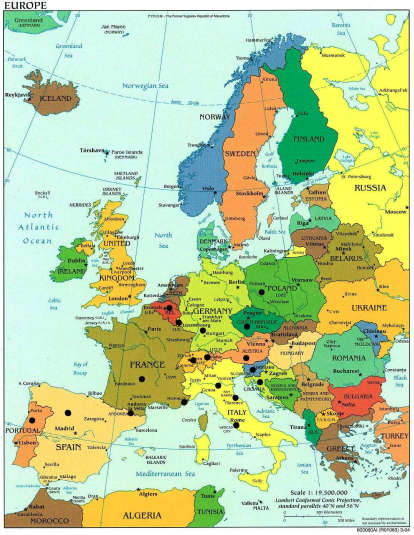
\includegraphics[width=\linewidth]{colormap.png}
    \caption{Four color map of Europe from Princeton University}
    \label{fig:fourcolor}
  \end{figure}

Figure \ref{fig:fourcolor} Four color of map of Europe from Princeton University

% %% ... the bibliography
\newpage
\bibliographystyle{acm}
\bibliography{biblio}

\end{document}

